\documentclass[aspectratio=169,11pt]{beamer}
\usetheme{Madrid}
\usepackage[T1]{fontenc}
\usepackage{lmodern}
\usepackage{amsmath,amssymb,mathtools,booktabs,array,tikz,mathrsfs}
\usetikzlibrary{arrows.meta,calc,positioning,backgrounds}
\definecolor{ink}{HTML}{162A3D}
\definecolor{teal}{HTML}{086B69}
\definecolor{clay}{HTML}{A34220}
\definecolor{muted}{HTML}{476073}
\definecolor{line}{HTML}{BACAD0}
\definecolor{paper}{HTML}{F5F8F8}
\setbeamercolor{normal text}{fg=ink,bg=white}
\setbeamercolor{structure}{fg=teal}
\setbeamercolor{palette primary}{fg=white,bg=teal}
\setbeamercolor{palette secondary}{fg=white,bg=teal!85!ink}
\setbeamercolor{palette tertiary}{fg=white,bg=ink}
\setbeamercolor{block title}{fg=white,bg=teal}
\setbeamercolor{block body}{fg=ink,bg=teal!5}
\setbeamerfont{frametitle}{size=\large,series=\mdseries}
\setbeamersize{text margin left=6.5mm,text margin right=6.5mm}
\setbeamertemplate{navigation symbols}{}
\setbeamertemplate{footline}{\leavevmode\hbox{\begin{beamercolorbox}[wd=.56\paperwidth,ht=2.7ex,dp=1.1ex,leftskip=6.5mm]{palette tertiary}\scriptsize Yihong Xiao\end{beamercolorbox}\begin{beamercolorbox}[wd=.44\paperwidth,ht=2.7ex,dp=1.1ex,rightskip=6.5mm plus 1fil]{palette primary}\hfill\scriptsize Lie Symmetry Reduction\end{beamercolorbox}}}
\setbeamertemplate{headline}{}
\setlength{\abovedisplayskip}{4pt}
\setlength{\belowdisplayskip}{4pt}
\newcommand{\source}[1]{\par\smallskip{\scriptsize\color{muted}#1\par}}
\newcommand{\lead}[1]{\textcolor{teal}{\textbf{#1}}}
\newcommand{\R}{\mathbb R}
\newcommand{\pr}{\operatorname{pr}}
\newcommand{\norm}[1]{\left\lVert#1\right\rVert}
\newcommand{\E}{\mathcal E}
\tikzset{arrow/.style={-{Latex[length=2mm]},line width=.8pt,draw=teal},
  flow/.style={draw=line,fill=paper,rounded corners=2pt,align=center,inner sep=4pt,font=\small},
  critical/.style={flow,draw=clay!70,fill=clay!6},
  plainline/.style={draw=muted,line width=.65pt}}
\title{Parameter-Dependent Lie Symmetries and Semi-Analytical Solutions of Nonlinear Partial Differential Equations}
\subtitle{Saint--Venant--Exner case studies}
\author{Yihong Xiao}
\institute{Mathematical Sciences, Wenzhou--Kean University\\Undergraduate Dissertation Defense\\Supervisor Dr. Puneet Rana}
\date{November 2026}
\begin{document}
% Spoken plan: 5 minutes 40 seconds + 20 seconds transition reserve.
% Frame 1, 0:15. My starting question was how changes in a constitutive
% parameter change the generators, and how an invariant equation becomes a
% usable reference solution. I study this through Saint-Venant-Exner systems.
\begin{frame}[plain]
\titlepage
\end{frame}

% Frame 2, 0:35. The water balances remain the same for any smooth flux of
% positive velocity. The two source papers use Eulerian and mass coordinates.
% Continuity defines the mass label. At fixed mass label the bed derivative
% includes an advection term. The compatible scalar restores that term,
% which is needed when checking the original balances.
\begin{frame}[t]{The governing equations and coordinate compatibility}
\small
\begin{columns}[T,onlytextwidth]
\column{.47\linewidth}
\lead{Eulerian SVE, $\E_1[Q]$}
\[
\begin{aligned}
 h_t+(hu)_x&=0,\\
 u_t+uu_x+g(h+B)_x&=0,\\
 B_t+D_xQ(u)&=0 .
\end{aligned}
\]
$h,u>0$, $g>0$. All quantities are dimensionless.
\[
 Q(u)=\kappa u^m,\quad m\ge1
\]
is the Grass-law case.
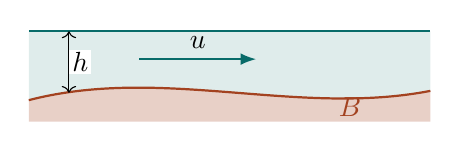
\begin{tikzpicture}[x=.85cm,y=.62cm]
\fill[teal!13] (0,1.85)--(6,1.85)--(6,.63)..controls(4,.1)and(2,1.15)..(0,.44)--cycle;
\fill[clay!25] (0,.44)..controls(2,1.15)and(4,.1)..(6,.63)--(6,0)--(0,0)--cycle;
\draw[teal,thick] (0,1.85)--(6,1.85);
\draw[clay,thick] (0,.44)..controls(2,1.15)and(4,.1)..(6,.63);
\draw[arrow] (1.65,1.28)--(3.4,1.28) node[midway,above]{$u$};
\draw[<->] (.6,.59)--(.6,1.85)node[midway,right,fill=white,inner sep=1pt]{$h$};
\node[clay] at (4.8,.3) {$B$};
\end{tikzpicture}
\column{.51\linewidth}
\lead{Material coordinate $s$}
\[
 \begin{gathered}ds=h(dx-u\,dt),\quad x=\phi(t,s),\\ b=B(t,\phi(t,s)).\end{gathered}
\]
\[
 \phi_s=1/h,\quad \phi_t=u,\qquad
 B_t\big|_x=b_t-\frac{\phi_t}{\phi_s}b_s .
\]
\lead{Grass-law scalars at matched parameters}
\[
 \boxed{\E_L[\phi]=\E_P[\phi]
 -D_s\!\left(\frac{\phi_t}{\phi_s}\mathcal A\right)}
\]
\scriptsize
\[
 \E_P=D_t\mathcal A-gm\kappa D_s T_m,
 \quad T_m=\phi_t^{m-1}\phi_{ts}/\phi_s.
\]
$\mathcal A=\phi_s\phi_{tt}-g\phi_{ss}/\phi_s^2$.
\par\smallskip
\scriptsize Recover fields by the inverse map and closed bed form.
\end{columns}
\source{(Paliathanasis, 2022; Paliathanasis, Leon and Leach, 2026)}
\end{frame}

% Frame 3, 0:45. A point symmetry is tangent to the equation in jet
% coordinates. Keeping the parameter symbolic gives a family of linear
% determining operators. Exact reduction needs a verified generator, rather
% than all inequivalent generators. In the Grass-law family the constraints
% are proportional to m minus three, and to m minus one for the printed
% scalar boost. Hence all nonexceptional real exponents share the same
% kernel, and an extra direction appears at an exceptional parameter.
\begin{frame}[t]{From continuous parameters to admitted generators}
\small
\[
 \boxed{\mathcal G(\mu)=\ker\mathscr D_\mu,\qquad
 \mathscr D_\mu X=\left.\pr^{(n)}X(\Delta_\mu)\right|_{\Delta_\mu=0}}
\]
$\mu=(g,\kappa,m)$, with $g,\kappa>0$, $m\in[1,\infty)$.
\begin{columns}[T,onlytextwidth]
\column{.53\linewidth}
\small For the extra scaling and boost coefficients $a_5,a_6$ the split determining equations give
\[
 \begin{array}{ll}
 \E_1,\E_L:&(m-3)a_5=0,\\
 \E_P:&(m-3)a_5=(m-1)a_6=0 .
 \end{array}
\]
Every real $m\ge1$ is included.
\column{.45\linewidth}
\centering
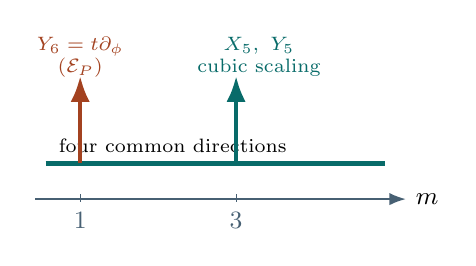
\begin{tikzpicture}[x=.88cm,y=.73cm,font=\small]
\draw[plainline,-{Latex}] (.35,.48)--(5.7,.48)node[right]{$m$};
\draw[teal,line width=2pt] (.5,1.1)--(5.4,1.1);
\node[anchor=west,font=\scriptsize] at (.55,1.4) {four common directions};
\draw[clay,line width=1.4pt,-{Latex}] (1,1.1)--(1,2.62);
\draw[teal,line width=1.4pt,-{Latex}] (3.25,1.1)--(3.25,2.62);
\node[font=\scriptsize,clay,align=center] at (1,2.95) {$Y_6=t\partial_\phi$\\($\E_P$)};
\node[font=\scriptsize,teal,align=center] at (3.58,2.95) {$X_5,\ Y_5$\\cubic scaling};
\foreach \x/\a in {1/1,3.25/3} {\draw[muted] (\x,.43)--(\x,.56) node[below=3pt] {$\a$};}
\end{tikzpicture}
\end{columns}
\begin{block}{Selection rule}
Select $\mathfrak h=\langle X\rangle\subset\mathcal G(\mu)$ with invariant graphs. Rank drops add directions.
\end{block}
\source{$X_5=t\partial_t-u\partial_u-2h\partial_h-2B\partial_B$, $Y_5=t\partial_t-2s\partial_s$. (Olver, 1993)}
\end{frame}

% Frame 4, 0:50. For arbitrary Q of positive velocity, autonomy and the
% dependence on derivatives of bed elevation imply that time translation
% and constant bed shift are symmetries. The combined generator gives a
% steady h and u and a constant bed drift. Mass, momentum and bed balance
% integrate immediately. The inverse function theorem gives an actual
% solution near any initial velocity where Q prime is nonzero. At a zero
% of Q prime a nonzero drift is impossible for a continuously differentiable
% profile. Thus classification of all additional symmetries is unnecessary.
\begin{frame}[t]{A reduction available for every smooth velocity flux}
For $Q\in C^2(I)$, $I\subset(0,\infty)$, autonomy and bed-shift invariance give
\[
 \boxed{T_\alpha=\partial_t+\alpha\partial_B\in\mathcal G[Q]},
 \qquad (h,u,B)=(H(x),U(x),Z(x)+\alpha t).
\]
Substitute this invariant graph into the three governing balances and integrate:
\[
 \boxed{HU=C,\qquad \frac{U^2}{2g}+H+Z=E,\qquad
 Q(U)=Q(U_0)-\alpha(x-x_0).}
\]
\begin{columns}[T,onlytextwidth]
\column{.50\linewidth}
\lead{When does a profile exist?}
\begin{itemize}\setlength{\itemsep}{3pt}
\item $Q'(U_0)\ne0$: unique local profile for fixed traces, by the inverse function theorem.
\item $Q'(U_0)=0$, $\alpha\ne0$: no $C^1$ profile at that trace.
\end{itemize}
\column{.47\linewidth}
\lead{Example beyond power laws}
\[
 Q(u)=e^u,\quad
 U(x)=\log(e^{U_0}-\alpha(x-x_0)).
\]
\[
 H=C/U,\quad Z=E-H-U^2/(2g).
\]
Valid locally where $U>0$.
\end{columns}
\source{Bed-drift family: Berthon et al. (2012). Here $C>0$ and $E$ fix the integration data.}
\end{frame}

% Frame 5, 0:35. The geometric requirement behind the previous graph is
% equal point and base orbit ranks. The quotient leaves d minus k variables.
% In a planar annulus rotation alone leaves time and radius. With a commuting
% time-bed drift the selected model has one radial variable. The annular
% first-order equation has a potentially vanishing leading coefficient,
% leading to a second type of singularity, distinct from the symmetry rank.
\begin{frame}[t]{Lie quotient and extension to a rotating annulus}
\begin{columns}[T,onlytextwidth]
\column{.44\linewidth}
\lead{Orbit geometry}
\centering
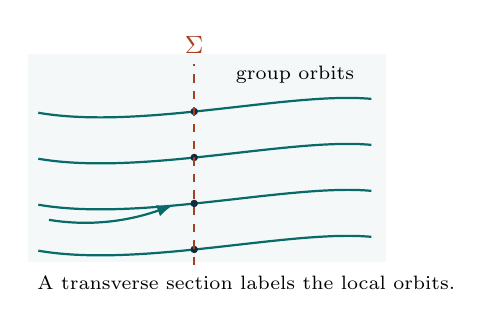
\begin{tikzpicture}[x=.9cm,y=.8cm]
\fill[paper] (.2,.3) -- (5.25,.3)-- (5.25,3.6)--(.2,3.6)--cycle;
\foreach \shift in {0,.73,1.46,2.19} {
 \draw[teal,thick] (.35,.48+\shift)..controls(1.8,.2+\shift)and(3.9,.82+\shift)..(5.05,.7+\shift);
 \fill[ink] (2.55,.50+\shift) circle (1.35pt);
}
\draw[clay,thick,dashed] (2.55,.25)--(2.55,3.44) node[above,font=\small] {$\Sigma$};
\draw[arrow] (.5,.97)..controls(1.15,.85)and(1.7,.98)..(2.25,1.2);
\node[font=\scriptsize,anchor=west] at (3.0,3.27) {group orbits};
\node[font=\scriptsize,anchor=west] at (.2,-.03) {A transverse section labels the local orbits.};
\end{tikzpicture}
\par\raggedright\small For a regular projectable action, equal point and base ranks $k$ leave $d-k$ variables.
\[
 \Delta\mapsto\mathcal R_{\mathfrak h}[\Delta]
\]
\column{.53\linewidth}
\lead{Planar model $\E_2$: rotation and bed drift}
\begin{columns}[c,onlytextwidth]
\column{.40\linewidth}
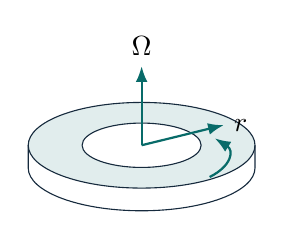
\begin{tikzpicture}[x=.72cm,y=.64cm]
 \fill[teal!12,even odd rule] (0,0)ellipse(2 and .85) (0,0)ellipse(1.05 and .44);
 \draw[ink] (0,0)ellipse(2 and .85);\draw[ink] (0,0)ellipse(1.05 and .44);
 \draw[ink] (-2,0)--(-2,-.45) arc[start angle=180,end angle=360,x radius=2,y radius=.85]--(2,0);
 \draw[arrow] (0,0)--(0,1.57)node[above]{$\Omega$};
 \draw[arrow] (0,0)--(1.45,.4)node[right]{$r$};
 \draw[arrow] (1.2,-.63)arc[start angle=-38,end angle=32,x radius=1.52,y radius=.67];
\end{tikzpicture}
\column{.57\linewidth}
\scriptsize Depth-averaged $(2+1)$ model with cubic flux and bed slope.
\end{columns}
\[
 (t,x,y)\xrightarrow{R}(t,r)
 \xrightarrow{T_c}r
\]
\small The second action is admitted for the nonexchange annular model; rotation alone gives a PDE.
\[
 \boxed{\Delta_c(r,H)H'=N(r,H)}
\]
\small A critical point requires compatibility of the vanishing coefficient and numerator.
\end{columns}
\source{(Olver, 1993; Dissertation, Ch. 3)}
\end{frame}

% Frame 6, 0:55. The solver first tests the leading matrix. If it is
% invertible and the right side is locally Lipschitz we have local existence.
% Otherwise the right side must lie in the image of the matrix; failure
% excludes C1 solutions. In a compatible singular case we seek analytic
% coordinates giving a Briot-Bouquet equation. If its linearization has no
% positive integer eigenvalues, the recurrence determines a unique convergent
% analytic germ. In the annular saddle, the opposite eigenvalue ratio makes
% the coefficient negative. Resonances or charts we cannot justify stay
% unresolved. This is the proposed general solver decision rule.
\begin{frame}[t]{Local solvability decides the solver branch}
\small
\begin{columns}[T,onlytextwidth]
\column{.45\linewidth}
\lead{Implicit reduced system}
\[
 M(z,Y)Y'=N(z,Y)
\]
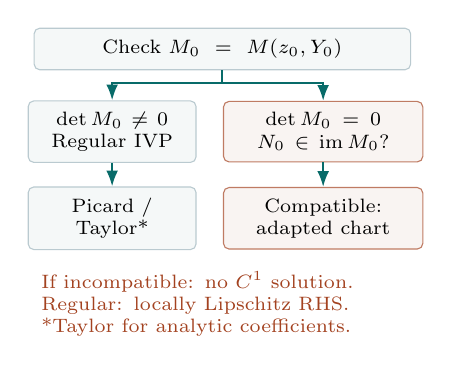
\begin{tikzpicture}[x=1cm,y=1cm]
\node[flow,font=\scriptsize,text width=4.5cm] (input) at (2.5,0) {Check $M_0=M(z_0,Y_0)$};
\node[flow,font=\scriptsize,text width=1.85cm] (regular) at (1.1,-1.05) {$\det M_0\ne0$\\Regular IVP};
\node[critical,font=\scriptsize,text width=2.25cm] (sing) at (3.78,-1.05) {$\det M_0=0$\\$N_0\in\operatorname{im} M_0$?};
\draw[arrow] (input.south)--++(0,-.16)-|(regular.north);
\draw[arrow] (input.south)--++(0,-.16)-|(sing.north);
\node[flow,font=\scriptsize,text width=1.85cm] (regout) at (1.1,-2.15) {Picard / Taylor*};
\node[critical,font=\scriptsize,text width=2.25cm] (test) at (3.78,-2.15) {Compatible: adapted chart};
\draw[arrow] (regular)--(regout);\draw[arrow] (sing)--(test);
\node[font=\scriptsize,clay,text width=4.6cm,align=left] at (2.5,-3.24) {If incompatible: no $C^1$ solution.\\ Regular: locally Lipschitz RHS.\\ *Taylor for analytic coefficients.};
\end{tikzpicture}
\column{.52\linewidth}
\lead{Briot--Bouquet criterion}
\[
 \rho w'=f(\rho,w),\quad w(0)=0.
\]
For holomorphic $f$, $f(0,0)=0$, set $J=\partial_w f(0,0)$. If
\[
 \boxed{\operatorname{spec}J\cap\mathbb N_{>0}=\varnothing},
\]
a unique analytic germ $w(0)=0$ exists.
\[
 (nI-J)a_n=b_n,\quad n\ge1.
\]
$b_n$ depends on lower coefficients.\\[2pt] Annular saddle: $J=\lambda_o/\lambda-1<-1$ (opposite-sign eigenvalues).
\par\smallskip
\textcolor{clay}{Resonance:} test $b_n\in\operatorname{im}(nI-J)$.
\end{columns}
\source{(Rong, 2013, Prop. 2.1; Dissertation, Chs. 3--4)}
\end{frame}

% Frame 7, 0:40. Once the analytic chart and trace are fixed, either
% a classical solver or the gated neural cell approximates its profile.
% For a self-mapping contraction, the integral defect is equivalent
% to solution error. That produces a continuous certificate when the
% defect norm can be enclosed. The neural benchmark used a sampled
% differential residual; the tank polynomial used integral defect.
\begin{frame}[t]{Approximation after analytic branch selection}
\centering
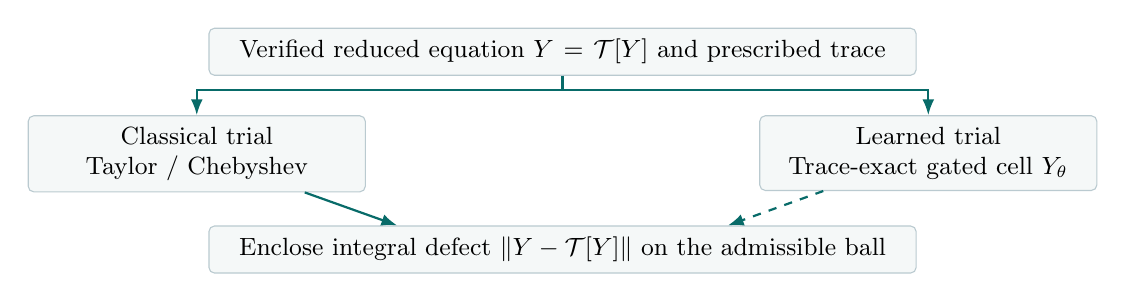
\begin{tikzpicture}[x=1cm,y=1cm]
\node[flow,text width=8.7cm] (data) {Verified reduced equation $Y=\mathcal T[Y]$ and prescribed trace};
\node[flow,text width=4.0cm,below left=5mm and -2cm of data] (classic) {Classical trial\\Taylor / Chebyshev};
\node[flow,text width=4.0cm,below right=5mm and -2cm of data] (ml) {Learned trial\\Trace-exact gated cell $Y_\theta$};
\draw[arrow] (data.south)--++(0,-.18)-|(classic.north);
\draw[arrow] (data.south)--++(0,-.18)-|(ml.north);
\node[flow,text width=8.7cm,below=19mm of data] (defect) {Enclose integral defect $\norm{Y-\mathcal T[Y]}$ on the admissible ball};
\draw[arrow] (classic)--([xshift=-2.1cm]defect.north);
\draw[arrow,dashed] (ml)--([xshift=2.1cm]defect.north);
\end{tikzpicture}
\par\smallskip
\begin{block}{Continuous certificate for a contraction}
If $\mathcal T:\mathcal B\to\mathcal B$ has Lipschitz constant $\Lambda<1$ and $Y\in\mathcal B$,
\[
 \boxed{\frac{\norm{Y-\mathcal T[Y]}}{1+\Lambda}
 \le \norm{Y-Y^*}\le
 \frac{\norm{Y-\mathcal T[Y]}}{1-\Lambda}} .
\]
\end{block}
\small The dashed route is proposed for learned trials; completed neural tests use sampled differential residuals.
\end{frame}

% Frame 8, 0:35. Four controlled sampled profile tests favor Chebyshev.
% The separate tank test has an exact linear offset equation; a degree-ten
% defect fit gives the displayed uniform bound and the five lifted balances
% are checked. These are concrete results, without claiming neural speedup
% or a certificate for the neural model. The nonlinear parameter sweep is
% the next matched-accuracy experiment.
\begin{frame}[t]{What the current computation establishes}
\begin{columns}[T,onlytextwidth]
\column{.55\linewidth}
\lead{Maximum sampled field error}
\medskip
\small
\begin{tabular}{@{}lrr@{}}
\toprule
Profile & Gated cell & Chebyshev\\\midrule
Eulerian drift & $6.07\cdot10^{-8}$ & $4.44\cdot10^{-16}$\\
Printed scalar & $1.30\cdot10^{-6}$ & $3.11\cdot10^{-15}$\\
Material wave & $7.64\cdot10^{-8}$ & $4.44\cdot10^{-16}$\\
Rotating exchange & $2.24\cdot10^{-6}$ & $1.22\cdot10^{-15}$\\
\bottomrule
\end{tabular}
\par\medskip
Chebyshev has the smaller sampled errors in all four tests. The fitted cell takes about $2$ s per task.
\column{.42\linewidth}
\lead{Separate certified tank profile}
\[
 b'=0.9-3b,\qquad b(0)=0.15.
\]
\begin{block}{Uniform offset error}
\[
 \norm{\widehat b-b^*}_\infty
 \le 4.762\times10^{-10}
\]
\scriptsize Degree-10 polynomial, rational Bernstein enclosure of its integral defect.
\end{block}
\small Three lifted balances vanish exactly; the remaining two residuals are continuously bounded.
\end{columns}
\source{Dissertation, Ch. 4: Tables 4.1--4.3. All quantities are dimensionless except runtime.}
\end{frame}

% Frame 9, 0:30. My conclusion is a composable method: find an admitted
% reduction, prove which local branch exists, approximate and reconstruct.
% For the velocity-flux SVE this always gives an available translation
% reduction, and regular initial data give nontrivial drifting-bed profiles.
% Future work is the harder functional group classification and automation
% of resonant and singular charts, followed by parameter-sensitive learning
% at matched certified accuracy.
\begin{frame}[t]{Conclusion and future work}
\begin{block}{Main result}
\[
 Q\ \text{or}\ \mu
 \ \longmapsto\ \mathcal G
 \ \supset\ \mathfrak h
 \ \longmapsto\ \mathcal R_{\mathfrak h}[\Delta]
 \ \longmapsto\ \text{solvability test}
\]
\end{block}
\lead{Established}
\begin{itemize}
\item A common Lie bed-drift reduction for autonomous SVE with arbitrary smooth $Q(u)$; local invertibility criterion.
\item Parameter-dependent Lie generators for every real Grass exponent $m\ge1$.
\item Regular and singular analytic profiles; a continuous tank defect certificate.
\end{itemize}
\lead{Future work}
\begin{itemize}
\item Full functional group classification $Q\mapsto\ker\mathscr D_Q$.
\item Automate adapted singular charts and resonance handling; compare parameter-sensitive learning at equal certified accuracy.
\end{itemize}
\source{Reproducibility: \href{https://github.com/CarlXerophilem/Lie-ML_PDES/tree/f498d648cce0633007430063bea008a2f4aac52a/delivery}{Lie--ML PDE Solver, pinned symbolic and numerical scripts}.}
\end{frame}
\end{document}
